\documentclass[a4paper,10pt,oneside]{book}
\usepackage[table,xcdraw]{xcolor}
\usepackage{graphicx}
\usepackage{float}
\usepackage{hyperref}
\usepackage[T1]{fontenc}
\usepackage[utf8]{inputenc}
\usepackage{setspace}
\usepackage[paper=a4paper,margin=1in]{geometry}
\usepackage{imakeidx}
\usepackage{tikz}
\usepackage{fancyvrb}
\usepackage{mathabx}

\makeindex

\begin{document}

    \begin{titlepage}
        
        \noindent
        \begin{minipage}[t]{0.19\textwidth}
            \vspace{-4mm}{\includegraphics[scale=1.15]{logo_unimib.pdf}}
        \end{minipage}
        \begin{minipage}[t]{0.81\textwidth}
        {
                \setstretch{1.42}
                {\textsc{Università degli Studi di Milano - Bicocca}} \\
                \textbf{Scuola di Scienze} \\
                \textbf{Dipartimento di Informatica, Sistemistica e Comunicazione} \\
                \textbf{Corso di laurea in Informatica} \\
                \par
        }
        \end{minipage}
        
	\vspace{40mm}
        
	\begin{center}
            {\LARGE{
                    \setstretch{1.2}
                    \textbf{Boh scrivici tipo esercizi di TCOM}
                    \par
            }}
        \end{center}
        
        \vspace{50mm}

        \vspace{15mm}

        \begin{flushright}
            {\large \textbf{Shitposter}} \\
            \large{Refolli Francesco} \\
            \large{Matricola 865955} 
        \end{flushright}
        
        \vspace{40mm}
        \begin{center}
            {\large{\bf Anno Accademico 2022-2023}}
        \end{center}

        \restoregeometry
        
    \end{titlepage}

\printindex
\tableofcontents

\part{Temi d'Esame 22/23}

\chapter{Gennaio 2023}

\section{Parte 1}

\subsection{Es 1}

Eseguo semplicemente la computazione della NDTM:

\begin{center}
    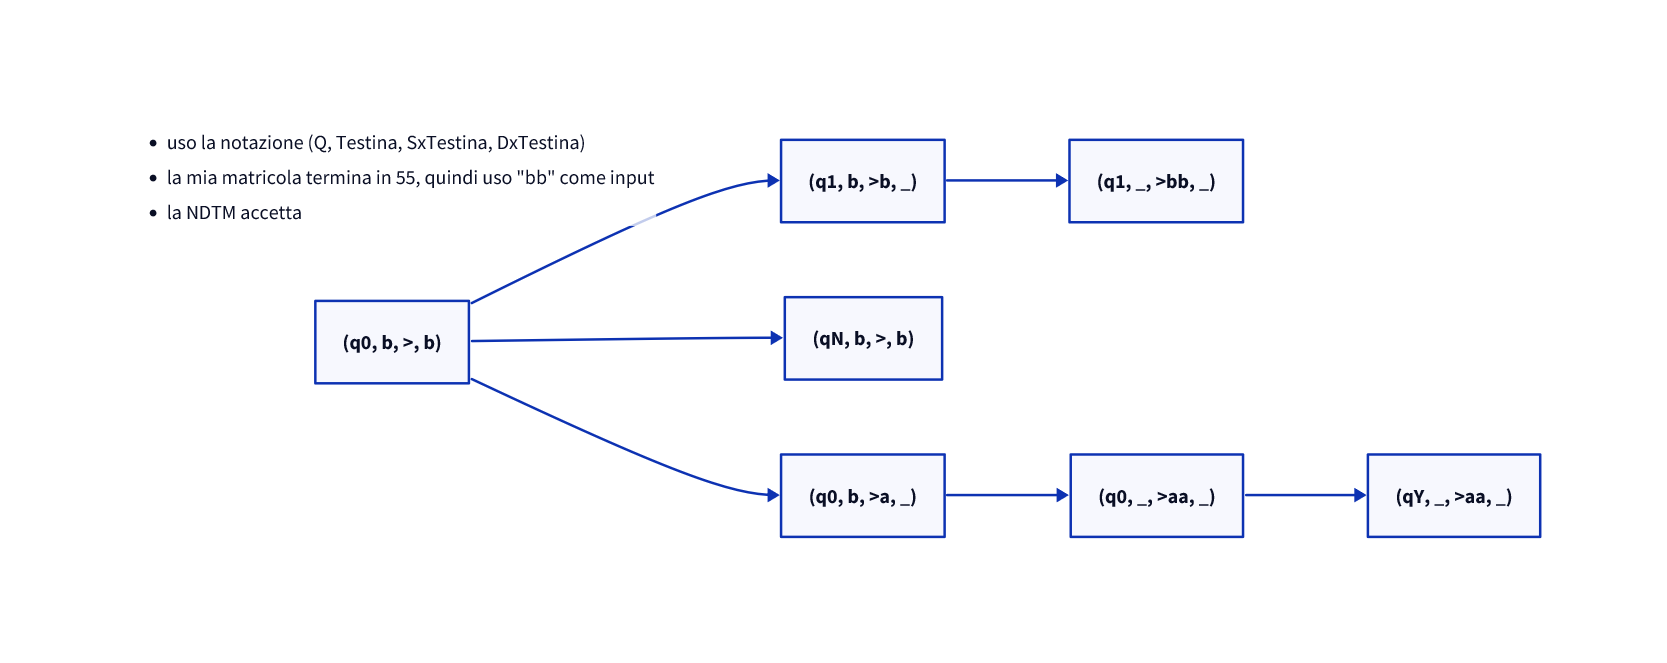
\includegraphics[width=1\linewidth]{Gennaio_01.png}
\end{center}

\subsection{Es 2}
\label{gennaio:1:2}

C'e' una lezione di Zandron che fa una roba del genere (crea una macchina magica D che non decide se stessa, ma non e' questo il caso. Qui e' molto piu' semplice.

Il ragionamento di Tizio e' sbagliato perche' prevede la ripetizione di una configurazione contando sul fatto che il numero totale di configurazioni sia limitato. Cio' pero' e' vero a prescindere solo su Macchine di Turing con spazio sul nastro limitato. Se il nastro e' illimitato (anche in una sola direzione) il numero possibile di combinazioni e' infinito, quindi e' possibile che una macchina di turing simulata vada in loop senza ripetere mai una volta una configurazione precedente.

Prendiamo per esempio la DTM che riscrive il simbolo che e' sotto la testina (blank o simbolo proprio) e si sposti a destra. Ogni spostamento produce una nuova configurazione, quindi non ripetera' mai una configurazione passata.

\subsection{Es 3}

Supponiamo che $\Pi \not \in NP$, allora $\Pi \in \overline {NP}$, ovvero non esiste una macchina di Turing non deterministica che risolva il problema $\Pi$ in tempo polinomiale. Sappiamo pero' per ipotesi che esiste una riduzione polinomiale $\Pi \leq SAT$, quindi e' possibile mappare un'istanza di $\Pi$ in una di $SAT$ in tempo polinomiale $F(n)$ e vice versa mappare una soluzione di $SAT$ a una di $\Pi$ sempre in tempo polinomiale $B(n)$. Se in primo luogo $SAT \in NP$, cioe' esiste una macchina NDTM che risolva SAT in tempo polinomiale $S(n)$, allora esiste una computazione in tempo polinomiale $T(n) = F(n) + S(n) + B(n)$ che risolva il problema di base $\Pi$. Quindi per assurdo $\Pi \in NP$.

\section{Parte 2}

Qui mi trovo molto in difficolta'. Per le riduzioni con Vertex Cover, Set Cover e Clique sto guardando \href{https://www.clear.rice.edu/comp487/VC\_Clique.pdf}{https://www.clear.rice.edu/comp487/VC\_Clique.pdf}

\subsection{Es 1.1}

Non ho capito cosa vuol dire 5-approssimante, pero' penso intenda il DTSP(k), cioe' TSP con al massimo peso $k = 5$. In questo caso prendo il grafo di partenza e etichetto ogni arco con peso $p = \frac {5} {|V|}$. Quindi applico $DTSP(k = 5)$ e trovo se esiste un ciclo di costo massimo 5 ($5 = p * |V|$) che attraversa i $|V|$ vertici, ovvero un ciclo Hamiltoniano (?!).

\subsection{Es 1.2}

%Riporto graficamente il grafo as-is: Gennaio_02.png

Again, per trovare un ciclo Hamiltoniano di minimo costo uso la riduzione polinomiale $HAM \leq TSP$. Dopo di che' il costo minimo e' 4 e il massismo e' 5.

Non e' una risposta rigorosa ma appunto non so come rispondere.

\chapter{Febbraio 2023}

\section{Part 1}

Per ora salto quelli spuri sull'esecuzione di TM perche' ne ho gia' fatto uno e sono una noia mortale.

\subsection{Es 1}

In breve la TM va a destra fino al primo blank sul primo nastro. Quindi torna indietro fino al triangolino di start sul primo nastro. Durante il ritorno scrive il simbolo che ha trovato sotto la testina del primo nastro sul secondo e si sposta a destra sul secondo.

Quando raggiunge il triangolino termina l'esecuzione.

Assumo la convenzione:
\label{tm:convenzione}
\begin{itemize}
    \item T sta per testina
    \item M sta per mossa
    \item S sta per mossa
    \item $\textvisiblespace $ sta per blank
    \item $\smalltriangleright$ sta per triangolino
    \item qY sta per mi fermo e accetto
    \item $\delta(S, T1, T2) \rightarrow (S', T1', T2', M1, M2)$
\end{itemize}

La funzione di transizione e':

\begin{itemize}
    \item $\delta(q0, a, \textvisiblespace ) \rightarrow (q0, a, \textvisiblespace , \rightarrow, -)$
    \item $\delta(q0, b, \textvisiblespace ) \rightarrow (q0, b, \textvisiblespace , \rightarrow, -)$
    \item $\delta(q0, \textvisiblespace , \textvisiblespace ) \rightarrow (q1, \textvisiblespace , \textvisiblespace , \leftarrow, -)$
    \item $\delta(q1, a, \textvisiblespace ) \rightarrow (q0, a, a, \leftarrow, \rightarrow)$
    \item $\delta(q1, b, \textvisiblespace ) \rightarrow (q0, b, a, \leftarrow, \rightarrow)$
    \item $\delta(q1, \smalltriangleright, \smalltriangleright) \rightarrow (qY, \smalltriangleright, \smalltriangleright, -, -)$
\end{itemize}

\subsection{Es 2}

Questo e' tipo una variante di \ref{gennaio:1:2}, ma piu' sofisticato. Qui si introduce un criterio di terminazione stringente.

Data una $M \in TM$, e un suo input $I$, allora

\begin{itemize}
    \item $M(I) \not = \perp$ in $k \leq n$ passi, ergo $(M,I) \not \in L$
    \item $M(I) \not = \perp$ in $k > n$ passi, ergo $(M,I) \not \in L$
    \item $M(I) = \perp$ in $+\infty$ passi, ergo $(M,I) \not \in L$
\end{itemize}

Quest'ultimo caso in particolare e' approssimabile al secondo. La macchina HPBT simula $O(n)$ passi e poi termina con $Y \oplus N$.

\begin{itemize}
    \item Per ogni $(M,I) \in L$, $HPBT(M, I) = Y$ quindi $L \in RE$.
    \item Per ogni $(M,I) \not \in L$, $HPBT(M, I) = N$ quindi $\overline L \in RE$.
    \item $L \in RE \land \overline L \in RE \Rightarrow L \in RIC$.
\end{itemize}

In alternativa si puo' ricordare che se il tempo e' limitato allora anche lo spazio e' limitato, perche' posso scrivere al massimo $k \leq n$ celle, quindi ho un numero limitato di configurazioni possibili. Quindi posso tenere traccia delle configurazioni gia' ottenute e terminare l'esecuzione se una configurazione e' ripetuta.

\subsection{Es 3}

Questo e' tipo una variante di \ref{gennaio:1:2}, ma piu' sofisticato. Qui si introduce una ipotesi importante: il nastro e' limitato. Potendo scrivere al massimo $n$ celle del nastro ho un numero finito di configurazioni possibili $|Q| * |\Sigma| * {|\Sigma|}^{n}$. Quindi posso tenere traccia delle configurazioni gia' ottenute e terminare l'esecuzione se una configurazione e' ripetuta.

\begin{itemize}
    \item Per ogni $(M,I) \in L$, $HPBS(M, I) = Y$ quindi $L \in RE$.
    \item Per ogni $(M,I) \not \in L$, $HPBS(M, I) = N$ quindi $\overline L \in RE$.
    \item $L \in RE \land \overline L \in RE \Rightarrow L \in RIC$.
\end{itemize}

\chapter{Giugno 2023}

\section{Part 1}

\subsection{Es 1}

No, prova con $bab$, finisce in un loop.

\subsection{Es 2}

Penso che sia l'esercizio di cui mi hai parlato dove Tizio inverte le uscite della NDTM e dice ok a posto. Nel mondo reale purtroppo non e' cosi' semplice.

Il problema principale e' che un problema e' in NP sse esiste una NDTM in grado di deciderlo in tempo polinomiale. Tuttavia se l'istanza-Y e' garantita essere polinomiale, questo non succede con l'istanza-N. Infatti se l'istanza-N non puo' essere risolta in tempo polinomiale da una NDTM allora il complementare di $\Pi$ non puo' essere parte di NP. Ovvero $\Pi$ non puo' essere in co-NP.

Un esempio di questi problemi non banali e' SAT. Se e' vero che e' possibile costruire e verificare un certificato in tempo polinomiale che dimostri che il problema ha soluzione, non e' possibile costruire e verificare un certificato polinomiale per dimostrare che un'istanza SAT non ha soluzione. L'unico modo per dimostrare che un'istanza non ha soluzione e' provare che tutte le $2^k$ combinazioni di assegnamenti per l'espressione non ha valore True. Questo certificato ha dimensione esponenziale. SAT non e' in co-NP.

Tizio deve andare nelle camere a gas.

\subsection{Es 3}

La riduzione avviene in tempo polinomiale perche' un ramo che terminerebbe in rifiuto viene semplicemente delayed su uno stato con mossa statica infinita ($(qk,s) \rightarrow (qk,s,-)$). Dopo di che' la riduzione all'istanza di Halting Problem e' corretta, perche' se N' non termina (ovvero rifiuta) allora anche $M_H$ rifiuta, e vice versa se una accetta allora accetta anche l'altra.

Il fatto che SAT sia NP-completo significa che $\forall P \in NP \Rightarrow P \leq SAT$, e se $SAT \leq HAL$ allora $\forall P \in NP \Rightarrow P \leq SAT \leq HAL \Rightarrow P \leq HAL$, quindi per definizione di NP-Hard, $HAL \in NP-Hard$.

\chapter{Luglio 2023}

\section{Part 1}

\subsection{Es 2.1}

Si, perche' per ogni $(M,I) \in L_H$, la macchina $M_H$ termina restituendo Y.

\subsection{Es 2.2}

Per esempio si prenda il problema complementare dell'Halting Problem, $\overline {L_H}$ dove $(M,I) \in \overline {L_H}$ sse $M(I) = \perp$. In questo caso non e' vero che $\forall (M,I) \in \overline {L_H} | M_H(M, I) = Y$.

\subsection{Es 3}

Tizio sbaglia: la costruzione dell'Array per Exists non avviene in tempo polinomiale. Detto $G = (V, E)$, il numero di sottografi $C_i$ possibili e' $2^{|V|}$, ovvero si impiegherebbe un tempo esponenziale per enumerare questi sottografi e comporre l'array. Quindi la riduzione e' legittima ma non e' polinomiale.

\section{Part 2}

Again non ho idea di cosa voglia dire 2-approssimante.

\part{Temi d'Esame 21/22}

\chapter{Febbraio 2022}

\section{Parte 1}

\subsection{Es 1}

Adotto le convenzioni \ref{tm:convenzione}.

\begin{itemize}
    \item $\delta(q0, 0) \rightarrow (q1, 0, \rightarrow)$
    \item $\delta(q1, 0) \rightarrow (qY, 0, \rightarrow)$
    \item $\delta(q1, 1) \rightarrow (q2, 1, \rightarrow)$
    \item $\delta(q2, 0) \rightarrow (q1, 0, \rightarrow)$
    \item $\delta(q2, 1) \rightarrow (q1, 1, \rightarrow)$
    \item $\delta(qY, 0) \rightarrow (q1, 0, \rightarrow)$
    \item $\delta(qY, 1) \rightarrow (q1, 1, \rightarrow)$
\end{itemize}

\begin{center}
    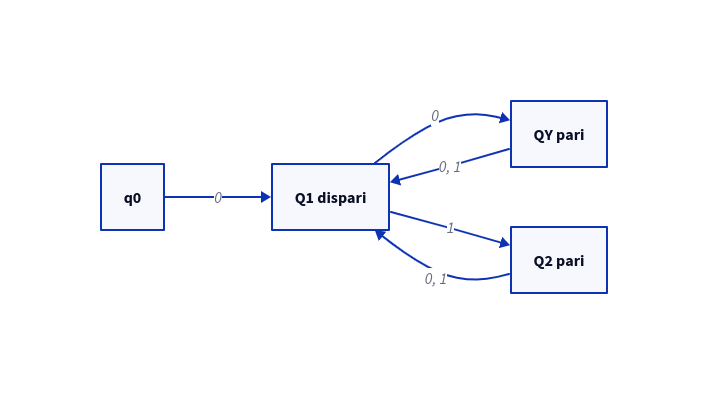
\includegraphics[width=1\linewidth]{22_febbraio_01.png}
\end{center}

\subsection{Es 2}

Boh l'avevo guardato ma non ci avevo capito nulla

\chapter{Giugno 2022}

\section{Parte 2}

\subsection{Es 2}

\begin{itemize}
    \item 1) Falso, tutti i problemi NP-Hard sono almeno difficili quanto i problemi NP, ma non sempre fanno parte di NP. Quando appartengono a NP si dicono NP-completi
    \item 2) Si, per definizione di problema NP-hard tutti i problemi NP si riducono polinomialmente ad esso
    \item 3) No, per definizione di NP-completo esiste una classe di problemi NP-Hard che appartengono ad NP, dove tutti i problemi in NP si riducono ad essi. Per il teorema di Cook-Levim, SAT e' un esempio di problema NP completo. 
\end{itemize}

\chapter{Luglio 2022}

\section{Parte 2}

\subsection{Es 2}

Dato un grafo $G = (V, E)$, si definisce ciclo Hamiltoniano un cammino $w = v_0,..,v_n$ tale che $set(w) = V$, $v_0 \equiv v_n$ e che $\forall v_i \in w \Rightarrow (v_i, v_{i+1}) \in E$.\\

Dato un grafo completo e pesato $G = (V, E, \delta)$, si definisce TSP il ciclo Hamiltoniano di costo minimo. In particolare $D-TSP(k)$ e' il problema decisionale associato a TSP parametrizzato $k \in R$, tale che il ciclo TSP abbia costo massimo $k$.\\

Data un'istanza di $HCP$ e' possibile fabbricare un'istanza di TSP manipolando la funzione di costo $\delta$. Si completa il grafo $G$ di partenza e si assegna un costo unitario agli archi presenti nel grafo di partenza. Quindi si etichettano i restanti archi con un numero piu' grande di 1, per esempio $k = 2$. Questa istanza di $D-TSP(|V|)$ risolve il problema di partenza.\\

E' possibile fabbricare un certificato polinomiale per dimostrare la soluzione per HCP: il ciclo stesso. Un verificatore puo' verificare il certificato in tempo polinomiale verificando che il cammino sia un ciclo e che visiti i nodi 1 volta ciascuno.

\chapter{Al so mia}

\section{Es 1}

Metto il testo qua perche' non ho voglia di cercarlo:

\begin{center}
    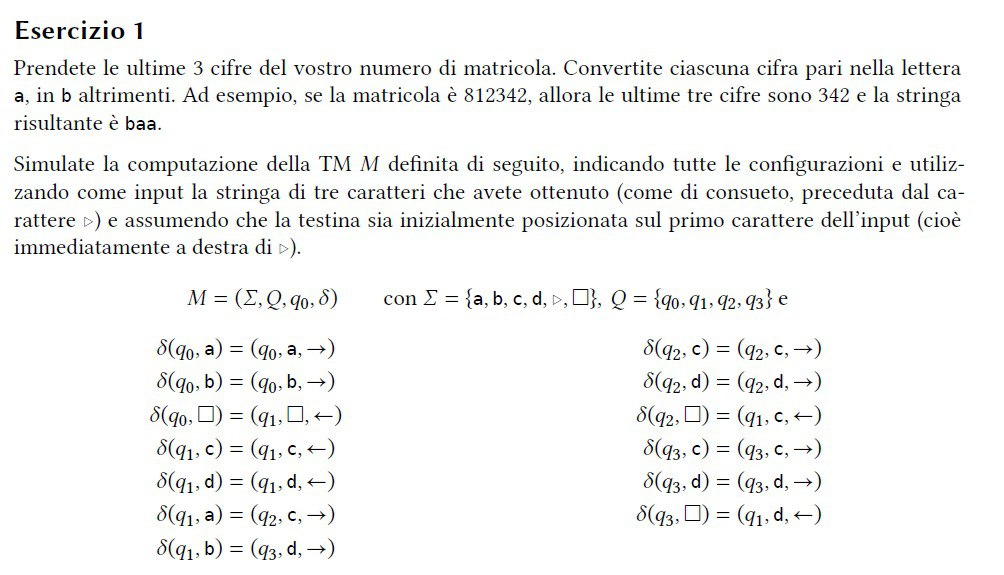
\includegraphics[width=1\linewidth]{photo_2023-11-13_17-24-47.jpg}
\end{center}

Indifferentemente dalla mia matricola, uso la sequenza $baa$ per DC.

\begin{itemize}
    \item $\overline b \; a \; a$
    \item $b \; \overline a \; a$
    \item $b \; a \; \overline a$
    \item $b \; a \; a \; \textunderscore$
    \item $b \; a \; \overline c$
    \item $b \; a \; c \; \overline c$
    \item $b \; a \; \overline c \; c$
    \item $b \; \overline c \; c \; c$
    \item $b \; c \; \overline c \; c$
    \item $b \; c \; c \; \overline c$
    \item $b \; c \; c \; c \; \overline c$
    \item $b \; c \; c \; \overline c \; c$
    \item $b \; c \; \overline c \; c \; c$
    \item $b \; \overline c \; c \; c \; c$
    \item $\overline d \; c \; c \; c \; c$
    \item $d \; \overline c \; c \; c \; c$
    \item $d \; c \; \overline c \; c \; c$
    \item $d \; c \; c \; \overline c \; c$
    \item $d \; c \; c \; c \; \overline c$
    \item $d \; c \; c \; c \; c \; \overline d$
    \item $d \; c \; c \; c \; \overline c \; d$
    \item $d \; c \; c \; \overline c \; c \; d$
    \item $d \; c \; \overline c \; c \; c \; d$
    \item $d \; \overline c \; c \; c \; c \; d$
    \item $\overline d \; c \; c \; c \; c \; d$
    \item $\overline \smalltriangleright \; d \; c \; c \; c \; c \; d$
    
\end{itemize}

\end{document}
